% Created 2024-03-06 Wed 11:48
% Intended LaTeX compiler: pdflatex
\documentclass[11pt]{article}
\usepackage[utf8]{inputenc}
\usepackage[T1]{fontenc}
\usepackage{graphicx}
\usepackage{longtable}
\usepackage{wrapfig}
\usepackage{rotating}
\usepackage[normalem]{ulem}
\usepackage{amsmath}
\usepackage{amssymb}
\usepackage{capt-of}
\usepackage{hyperref}
\usepackage{placeins}
\usepackage{gensymb}
\usepackage{tabularx}
\author{Christian Johnson\and\&\and Dan Nusraty\and\&\and Dylan Mcgill\and \newline \uline{Optimail}}
\date{\today}
\title{Mail Database Project}
\hypersetup{
 pdfauthor={Christian Johnson\and\&\and Dan Nusraty\and\&\and Dylan Mcgill\and \newline \uline{Optimail}},
 pdftitle={Mail Database Project},
 pdfkeywords={},
 pdfsubject={},
 pdfcreator={Emacs 29.2 (Org mode 9.6.15)}, 
 pdflang={English}}
\begin{document}

\maketitle

\section{Contents}
\label{sec:org5b9eeda}
\subsection{Functional Requirements}
\label{sec:org4d06cec}
\subsection{Non Functional Requirements}
\label{sec:orgefc45a3}
\subsection{Use Case Diagram}
\label{sec:orgc6c622c}
\subsection{Meeting Summaries}
\label{sec:org0018a43}
\subsection{Individual Use Cases}
\label{sec:org27816d4}
\subsubsection{Dan}
\label{sec:org87cd082}
\subsubsection{Christian}
\label{sec:org8380ec5}
\subsubsection{Dylan}
\label{sec:orgb3cce39}
\clearpage
\section*{Functional Requirements}
\label{sec:orgbbb587b}
\begin{itemize}
\item System will accept data entry
\item System will record tracking number and addressed box number for incoming packages
\item System will add entered information into sql database
\item System will associate incoming packages with Cadet information based on addressed box number
\item System will notify Cadet upon package arrival
\item System will record package status (Picked up or not)
\item Users can search database for packages
\item System will display all packages matching search terms
\item Users can easily update package status
\item Developers will write code in an organized fashion, such that the system is easy to expand later.
\item System will allow user to categorize packages (e.g. perishable, priority, regular)
\item System will authenticate users with a login screen. Certain functionality wil only be available to users with authentication
\item System will record a history of package movement and status change
\item System will provide reporting tools to the user
\item System will feature a status dashboard to show totals and informational breakdowns.
\end{itemize}
\section*{Non Functional Requirements}
\label{sec:orga1c63aa}
\begin{itemize}
\item Will not misassociate packages
\item Will allow package entry, given necessary data, within 5 seconds
\item Will be easily navigable, with all system functions available within 5 clicks
\item Will allow package retrieval, given sufficient search information, within 10 seconds
\item Will never fail to retrieve Cadet information, given sufficient correct search information
\item Will never allow a package entry without associated Cadet information and association
\end{itemize}

\section*{Use Case Diagram}
\label{sec:org8e29a86}

\begin{figure}[htbp]
\centering
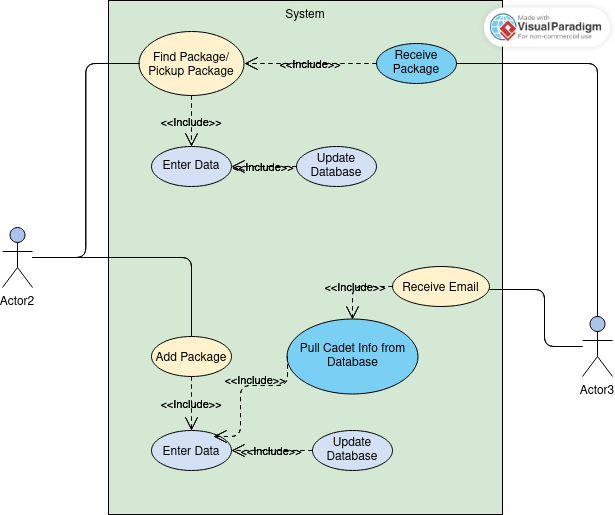
\includegraphics[width=.9\linewidth]{/home/csj7701/Projects/Mail-Database-Project/Class-Documents/Requirements_UseCaseDiagram.png}
\bicaption{.                        Actor 2: Employee, Actor 3: Cadet }
\end{figure}
\newpage
\section*{Meeting Summaries}
\label{sec:orge84832f}
\subsection*{Meeting 1 - 30JAN2024}
\label{sec:orge9e4e30}
\begin{itemize}
\item Decided on division of labor
\item Agreed on general project scope
\item Began formulating Functional Requirements
\end{itemize}
\subsection*{Meeting 2 - 01FEB2024}
\label{sec:orgccd4ad5}
\begin{itemize}
\item Created Use-Case Diagram
\item Finished Functional Requirements
\item Started Non Functional
\item Started individual Use Cases
\end{itemize}
\subsection*{Meeting 3 - 02FEB2024}
\label{sec:org39d4412}
\begin{itemize}
\item Polished Use-Case Diagram
\item Completed Requirements
\item Finished Individual Components
\end{itemize}

\section*{Individual Use Cases}
\label{sec:orgf4218ee}

% DAN
\newpage
\begin{table}[tbp]
\vskip-1.0cm\hskip-3.0cm\begin{tabularx}{1.5\textwidth}{|X|X|}
\hline\multicolumn{2}{|c|}{UC01 - Retrieve Package (Dan)} \\
\hline Scope & Package Notification System \\
\hline Level & User Goal \\
\hline Primary Actor & Cadet \\
\hline Stakeholders and Interests & Cadet: The cadet wants a simple and effective way to get their package \\ & Employee: wants a simple and effective way to find and deliver necessary packages. \\
\hline Preconditions & Cadet receives an email indicating a package is ready \\
\hline Postconditions & Cadet leaves the mailroom with their package. Mailroom staff updates the database, package is marked as delivered. \\
\hline Main Success Scenario & 1. Cadet receives an email notifying them of a package \\
& 2. Cadet arrives at mailroom and requests package \\
& 3. Mailroom conducts "Find Package/ Pickup Package" to retrieve the package. \\
& 4. Cadet takes custoody of their package from mailroom staff. \\
\hline Extensions & 1A. Cadet does not see notification email (did not receive, or simply didn't notice) \\
& 1Ai. In case of a database issue, mailroom staff should be notified.  \\
& 1Aii. Cadets should resolve issues with their own email themselves \\
& 1Aiii. In either case, the mailroom will still have the package; the cadet must then manually check whether a package is there. \\
& 2A. If the cadet does not arrive at the mailroom, the package will be retained indefinitely either until it is retrieved or the addressee graduates. \\
& 3A. If the mailroom fails to locate the package, they must check logs and records that are seperate from this system in order to locate it. \\
\hline Special Requirements & The cadet must receive a package, and be willing to go to the mailroom to pick it up. \\
\hline Technology and Data Variations & Touchpad to sign for package \\
\hline Frequency of Occurence & Nearly Continuous \\
\hline
\end{tabularx}\end{table}
% CHRISTIAN

\begin{table}[tbp]
\hskip-3.0cm\begin{tabularx}{1.5\textwidth}{|X|X|}
\hline
\multicolumn{2}{|c|}{UC02 - Find Package (Christian)} \\
\hline
Scope & SQL Mail Database \\
\hline
Level & User Goal \\
\hline
\Primary Actor & Mailroom Staff \\
\hline
\stakeholders and Interests & Mailroom Staff: Want effificient and simple query methods \\ & Cadets: Want staff to find their package quickly \\
\hline
Precondition & Mailroom has package \\ & Package properly stored in database \\ & Mailroom has correct Cadet info for search \\
\hline
Postconditions & Package information updated in database \\
\hline
Main Success Scenario & 1. Cadet arrives at mailroom \\ &
2. Mailroom staff enters Cadet info \\ & 3. all relevant results are displayed \\
& 4. Mailroom staff retrieves package \\ & 5. Cadet receives package and leaves \\
& 6. Database updated \\
\hline
Extensions & 3a. No results, mailroom staff checks the email sent to the cadet (should contain information to find the package manually) \\
\hline
Special Requirements & None \\
\hline Technology and Data & None \\
\hline Frequency & Nearly Continuous \\
\hline Open Issues & None \\
\hline \end{tabularx} \end{table}

% DYLAN

\begin{table}[tbp]
\vskip-2.0cm\hskip-3.0cm\begin{tabularx}{1.5\textwidth}{|X|X|}
\hline
\multicolumn{2}{|c|}{UC03 - Add Package (Dylan)} \\
\hline
Scope & SQL Mail Database \\
\hline
Level & System goal \\
\hline
Primary Actor & Mailroom Staff \\
\hline
Stakeholders and Interests & Mailroom Staff: Want efficient and streamlined storage of packages \\
 & Cadet: Wants timely and accurate notification of package receipt \\
\hline
Precondition & Package has been physically received by the mailroom staff \\
\hline
Postconditions & Package information has been added to SQL Database \\
 & Email notification has been sent to Cadet \\
 & Package has been stored appropriately \\
\hline
Main Success Scenario & 1. Mailroom staff scans the package \\
 & 2. Automated system scans the package and reads tracking number/box number \\
 & 3: Package status is updated in database along with timestamp and date \\
 & 4. System generates and sends an email to Cadet \\
 & 5. Staff stores the package in appropriate area/box number \\
\hline
Extensions & 1a. Invalid/incomplete information \\
 & 1. Mailroom staff notified, providing option to manually input information \\
 & 3a. Database upload failure \\
 & 3. Mailroom staff notified, given guidance on resolving the issue \\
 & 4a. Email notification failure \\
 & 4. Mailroom staff notified, given guidance on resolving the issue \\
 & Cancel Operation: Mailroom staff may cancel the operation at anytime \\
\hline
Special Requirements & Secure database is used to protect cadet security \\
\hline
Technology and Data & {empty} \\
\hline
Variations List & 1a. Automated scanning system \\
 & 3a. SQL Database \\
 & 4a. Email notification system \\
\hline
Frequency of Occurrence & Regularly: Anytime the mailroom receives a package \\
\hline
Open Issues & Ensure seamless integration with current scanners \\
 & User training \\
 & Systems ability to handle high volume of packages during highly busy times \\
\hline
\end{tabularx}
\end{table}
\end{document}
